
\documentclass[12pt,a4paper,titlepage,oneside]{article}

\usepackage{po}
\sloppy

\headline{Prüfungsfragen}
\subtitle{Robotik und Automation in der KFZ-Elektronik}
%\definecolor{highlight}{rgb}{0,.6,0} 

\begin{document}

\maketitle

\section{Einführung}
-

%%%%%%%%%%%%%%%%%%%%%%%%%%%%%%%%%%%%%%%%%%%%%%%%%%%%%%%%%%%%%%%%%%%
% A.2
%%%%%%%%%%%%%%%%%%%%%%%%%%%%%%%%%%%%%%%%%%%%%%%%%%%%%%%%%%%%%%%%%%%
\section{Industrieroboter}

\subsubsection*{Beschreiben Sie die Teilsysteme eines Industrieroboters und deren Funktion 
  (S.6,20)}
\begin{description}
\item[Kinematik:] bewegt die Fertigungseinrichtung zum Werkstück (räumliche Zuordnung zw. 
  Werkstück und Fertigungseinrichtung); besteht aus Achsen, Antrieben, internen Sensoren, 
  Effektoren;
\item[Antrieb:] Übertragung/Umwandlung der Energie bis hin zum Effektor
\item[Steuerung:] Umsetzung des Anwenderprogramms in eine Bewegung; Ein- und Ausgabeoperationen
  zur Steuerung von Abläufen; Informationseingabe und -speicherung;
\item[Messsystem:] Lage- und Geschwindigkeitmessungen der Achsen
\item[Effektor:] Werstück-, Werkzeug-, Prüfmittelaufnahme
\item[Externe Sensoren (optional):] Toleranzausgleich (zB: Kamera überprüft Abstand zum 
  Werkstück); Lage- und Mustererkennung; 
\end{description}

\subsubsection*{Beschreiben Sie die Bauformen von Industrierobotern (S.7)}
\begin{description}
\item[Portalroboter:] steife Struktur; rechteckiges oder quaderförmiges Industrieportal; 
  für große Arbeitsbereiche; Anw.: Transport von schweren Lasten, Verkettung von 
  Fertigungseinrichtungen;
\item[Roboter mit Lineararmen auf Schienen:] Lineararme meist in kartesischem Koordinatensystem
  angeordnet; Anw.: Einlegeoperationen, Punktschweißen;
\item[Schwenkarmroboter:] erste Achse ist Drehachse;
\item[Horizontalknickarmroboter (SCARA):] Achsen stehen senkrecht; Vorteil: billig, schnell, 
  genau!
\item[Vertikalknickarmroboter:] Achsen stehen horizontal (Abknicken in vertikaler Ebene 
  $\rightarrow$ Bremsen notwendig);
\end{description}
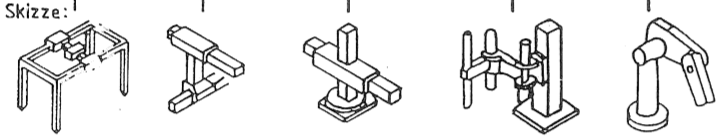
\includegraphics[width=\textwidth]{pics/bauarten}

\subsubsection*{Nennen Sie Beispiele für Effektoren. Welche Vor- bzw. Nachteile haben pneumatische 
Greifer? (S.8,9,29-34)}
3 Arten: Greifer (Montage, Handhabung), Werkzeug (Schweißen, Schraubenzieher, Lackpistole), 
Prüfmittel (Sensoren)
\begin{description}
\item[Standardgreifer:] zwei ``Finger''/Backen, die ein Werkstück greifen; Hier kann mann noch
  zwischen \emph{pneumatischen} und \emph{elektromotorischen} Greifern unterscheiden:
  \begin{description}
    \item[pneumatisch:] + Greifkraft positionsunabhängig (konstant); - Nothaltevermögen durch
      zusätzliche Federn; + zentrieren Teile; - bewegliche Backen führen dazu, dass die 
      Position der Teile am Greifer nicht genau definiert ist;
    \item[elektromotorisch:] + Lageregelung (vgl. Nachteil bei pneumatisch) $\rightarrow$ 
      flexibler; + Greifkraft variabel (vgl. schwere vs. zerbrechliche Teile)
  \end{description}
\item[Sonderbacken:] + flexibler; Unterteilung in: Teilefamilienbildung (alle Werkstücke haben 
  eine best. Fläch wo der Backen das Teil aufnehmen kann), Stufengreifer (unterschiedliche
  Öffnungsweiten der Backen), Revolvergreifer (mehrere Teile auf einmal aufnehmen 
  $\rightarrow$ kürzere Taktzeiten), Greiferwechsel, Fingerwechsel
\item[Sauggreifer:] Werkstücke mit Unterdruck ansaugen; Anw.: Leiterplattenbestückung;
\item[Sonderbauformen:] Mehrfachgreifer, Kunststoffgreifer
\item[Werkzeugwechselsysteme:] Roboter wechselt die Greifer; - lange Taktzeiten;
\end{description}

\subsubsection*{Nennen Sie Kriterien zur Auswahl eines Werkzeugwechselsystem. (S.34)}
Zulässige Kräfte und Momente, Anzahl der Steueranschlüsse, Anzahl der unterscheidbaren 
Werkzeuge, Einfahrtoleranzen, Spielfreiheit, Nothaltevermögen, Gewicht, Abmessungen, Preis

\subsubsection*{Beschreiben Sie die verschiedenen Steuerungsarten von Industrierobotern. Zeichnen
  Sie eine Beispielskizze für die resultierende Bahn zwischen 2 Punkten bei einem 
  Industrieroboter mit 2 rotatorischen Achsen. (S.9,35-37)}
\begin{description}
\item[Punkt-zu-Punkt (PTP):] 2 Punkte gegeben $\rightarrow$ Winkel der Achsen werden 
  zurückberechnet (=Rückwärtskinematik) $\rightarrow$ Achsen bewegen sich unabhängig 
  voneinander zu den berechneten Winkeln (kann auch gleichzeitig/synchron erfolgen);
\item[Vielpunkt-Steuerung (MP):] Sollwerte/Punkte in festem Zeitraster vorgegeben (sonst
  wie PTP);
\item[Bahnsteuerung (CP):] mathematische Darstellung der Bahn, meist auch mit 
  Geschwindigkeitsvorgaben; alle Achsen bewegen sich synchron mit berechneten Achswinkeln;
\end{description}
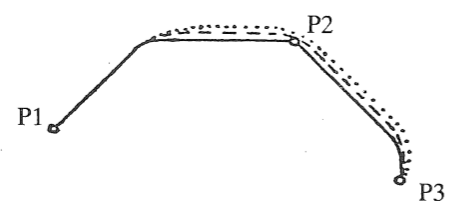
\includegraphics[width=.4\textwidth]{pics/ptp_bsp}

\subsubsection*{Was versteht man unter Folgeprogrammierung? Beschreiben Sie Vor- und Nachteile
  im Vergleich zu Off-line-Programmierung. (nicht gefunden) \\ bzw. \\
  Was versteht man unter Teach-In Programmierung? Beschreiben Sie Vor- und Nachteile im 
  Vergleich zu Off-line-Programmierung. (S.10,38)}
\begin{description}
\item[Einstellverfahren:] Punkte oder Bahn im Zeitraster einfach übernehmen (händisch, taktil,
  oder optisch positionieren); + schnell; + einfach; - ungenau;
\item[Master-Slave:] Einstellen des Roboters mithilfe eines kleineren Master-Roboters 
  (händisch); 
\item[Teach-In:] Positionierung mit Handbediengerät; 
  - aufwendig; + genau (jeder Roboter ist anders! $\rightarrow$ hier: relative
  Genauigkeit miteinbezogen); - Roboter fällt für die Zeit des Teach-In's aus!
\item[Off-Line:] + textuelle Programmierung Off-Line (Roboter muss nicht für die Produktion 
  ausfallen); Simulation der Bewegung mit CAD-Daten; - ungenau, weil nur absolute Genauigkeit 
  des Roboters verwendet wird;
\end{description}
Folgeprogrammierung = Master-Slave??


%%%%%%%%%%%%%%%%%%%%%%%%%%%%%%%%%%%%%%%%%%%%%%%%%%%%%%%%%%%%%%%%%%%
% A.3
%%%%%%%%%%%%%%%%%%%%%%%%%%%%%%%%%%%%%%%%%%%%%%%%%%%%%%%%%%%%%%%%%%%
\section{Toleranzausgleich, Sensorik, Bewegungsführung}

\subsubsection*{Beschreiben Sie die zwei prinzipiellen Methoden zum Toleranzausgleich und 
  nennen Sie Beispiele. (S.42,45)}
\begin{description}
\item[aktiv:] Roboter nachjustieren/positionieren; Bewegungsführung; 

  Bsp. 1: Stift in eine
  Bohrung setzen $\rightarrow$ mit Sensor Bohrung \emph{suchen} (laufendes Erfassen während 
  Bewegung) oder \emph{messen} (Momentaufnahme); 

  Bsp. 2: Bauteil für LP-Bestückung aufnehmen
  $\rightarrow$ Momentaufnahme/Bild von Sauger und Bauteil machen (Position messen) und 
  anschließend zentrieren
\item[passiv:] Toleranz verursacht ``elastische Verformung''; nachgiebige Regelung; 

  Bsp.: Stift in eine Bohrung
  setzen $\rightarrow$ Werkstück so gestalten, dass die Toleranz eine Kraft hervorruft und 
  den Greifer \emph{passiv} bewegt (keine Ecken, sondern Schrägen - hier: angefaster Stift
  und Bohrung)
\end{description}

\subsubsection*{Beschreiben Sie das Prinzip der Sensorführung von Industrierobotern. Unter
  welchen Bedingungen ist Sensorführung sinnvoll? Welche Probleme sind dabei zu beachten? 
  (S.42,50)}
Prinzip: Abweichung zwischen Effektor und Werkstück messen/suchen $\rightarrow$ Rückführung
an Steuerung $\rightarrow$ Auswertung und Regelung der Achsen/Antriebe

Sinnvoll wenn: Bewegung störanfällig oder komplex (Korrektur der Bahn mit Sensoren), 
große Werkstücktoleranzen, hohe Genauigkeitsanforderungen, biegeschlaffe Werkstücke, 
keine geordnete Bereitstellung möglich (vgl. Stapel von Scheiben für die Montage in ein
Fahrzeug), ... (S.50)

Probleme: - zusätzlicher Engineering-Aufwand (Regelung anstatt ``nur'' Steuerung); - keine
einheitlichen Sensorschnittstellen vorhanden; - hohe Sensorkosten; - geringe 
Systemverfügbarkeit; - mangelnde Fähigkeiten der Steuerungen zur Umsetzung von
Sensorsignalen in Bewegungsmodifikationen; - unzureichende dynamische Eigenschaften der 
Steuerungen


\end{document}

